% Martin Rodriguez Jr.
% SID: 811958765


%Anything following a % sign is a comment.
%Please use the comments to help you understand the code below.

%%%%%%%%%%%% Quick Notes %%%%%%%%%%%%%%%%%%%%%%

% \textit{} ==> italicises words or phrases
% \textbf{} ==> bolds words or phrases
% \\ ==> creates a new line
% \S ==> creates section section symbol, fancy double s thing
% \renewcommand{\baselinest8retch}{2} ==> double spaces the document

%%%%%%%%%%%%%%%%%%%%%%%%%%%%%%%%%%%%%%%%
\documentclass[12pt]{article}

%LOAD VARIOUS PACKAGES
\usepackage{setspace}
\usepackage{caption}
\usepackage{subcaption}
\usepackage{graphics, latexsym, multicol}		%
\usepackage{graphicx}
\usepackage{lscape}

\usepackage{amsmath, amsfonts, amsthm, amssymb}		%Math packages provided by American Math Society (AMS)
\usepackage{thmtools}

\usepackage{xcolor}							%Extended color package: provides colors for text enhancement
%\usepackage[margin = 1.00in, top = 1in, bottom = 1in, nohead] {geometry}
\usepackage{boxedminipage}					%allows use of boxed minipages
\usepackage{enumitem}


\usepackage[english]{babel}
\usepackage{xcolor} % Required for specifying custom colors
\usepackage{fix-cm} % Allows increasing the font size of specific fonts beyond LaTeX default specifications

\usepackage{longtable}

%MATH CHARACTER COMMANDS: Short hand for commands
\def\N{\mathbb{N}}		 				%Natual Bold Face: \N is now the command for the Natural Numbers
\def\Q{\mathbb{Q}} 						%Rational Bold Face: \R
\def\R{\mathbb{R}} 						%Real Bold Face
\def\Z{\mathbb{Z}} 						%Integers Bold Face
\def\C{\mathbb{C}} 						%Complex Bold Face
\def\eps{\varepsilon}                                               % Defines \varepsilon to \eps
\renewcommand{\qedsymbol}{$\blacksquare$} % QED symbol

\def\L{\mathcal{L}}



%Solution template with little sideways triangle
\declaretheoremstyle[
spaceabove=6pt, spacebelow=6pt,
headfont=\normalfont\bfseries,
notefont=\mdseries, notebraces={(}{)},
bodyfont=\normalfont,
postheadspace=1em,
numberwithin=section
]{exstyle}
\declaretheoremstyle[
spaceabove=6pt, spacebelow=6pt,
headfont=\normalfont\bfseries,
notefont=\mdseries, notebraces={(}{)},
bodyfont=\normalfont,
postheadspace=1em,
headpunct={},
qed=$\blacktriangleleft$,
numbered=no
]{solstyle}
\declaretheorem[style=exstyle]{example}
\declaretheorem[style=solstyle]{solution}

%\newenvironment{solution}
%  {\begin{proof}[Solution]}
%  {\end{proof}}
%
%



\usepackage{hyperref}
\usepackage{listings}


\begin{document}

\begin{center}
	{\LARGE Homework 4} \\[10pt] 
	{ Martin Rodriguez} \\
	Student ID: 1151332\\
	AMS 209: Foundations of Scientific Computing\\
	Professor Dongwook Lee\\[10 pt]	
	31 October 2017 {\tiny boo!} \\[30 pt]
\end{center}


\section*{{\large Problem 1: Website}}

Website Link = \href{https://people.ucsc.edu/~mrodrig6/}{Click Here.}


\section*{{\large Problem 2: Newton Root Finder}}

\begin{enumerate}
	\item In this exercise, I have modified a couple of bits in file `\texttt{RootFinder.F90}'. I added a `\texttt{ftnType}' to line 34 so the driver file knows which function is being used. This then allows us to print the target function. I added the printing commands between lines 67-79 in `\texttt{RootFinder.F90}'.
	
	\item I have added the print commands between lines 57 and 67 in file \texttt{setup\_module.F90}.
	
	\item For this exercise, we had to plot the target function, roots and the initial guess. It is shown in figure \ref{fig:plot2dot3}.
			\begin{figure}[h]
				\caption{The target function $f(x) = (x-1)(x-2)$.}
				\centering
				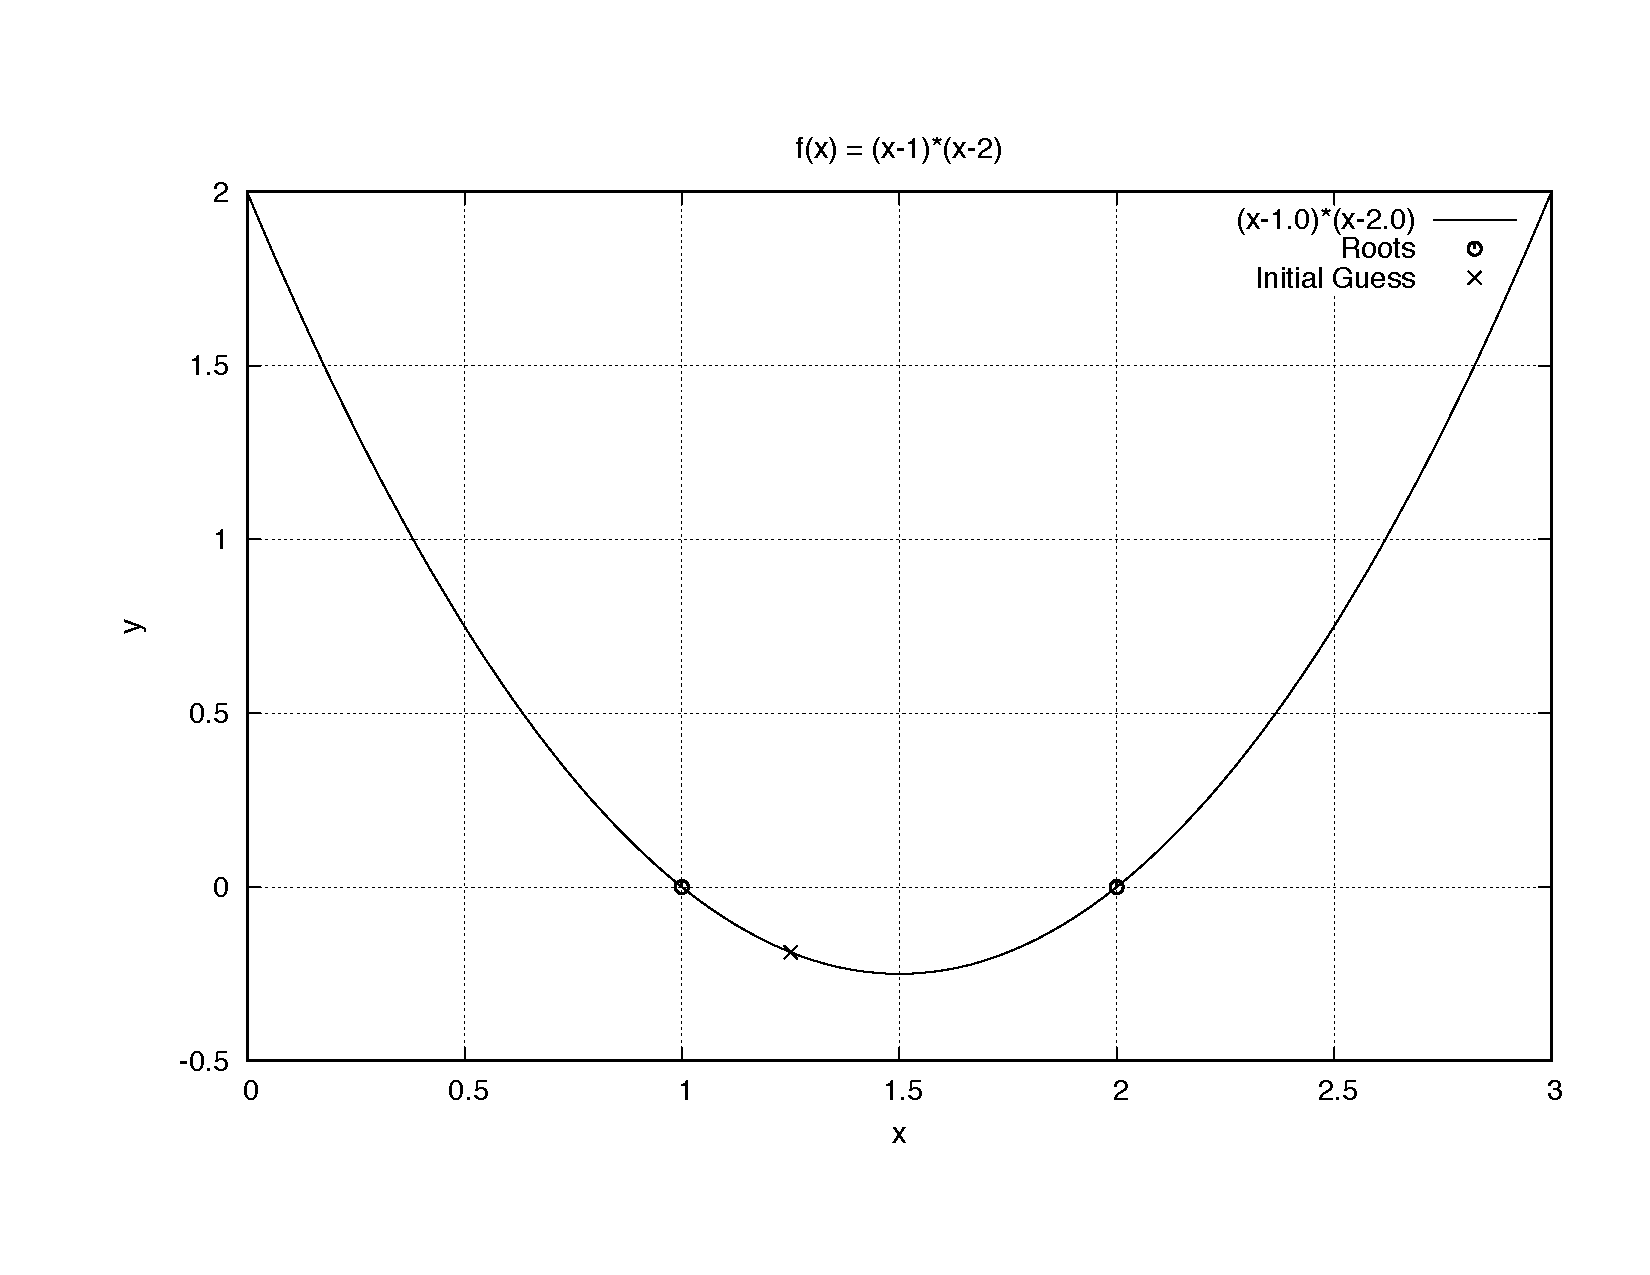
\includegraphics[width=0.85\textwidth]{./problem2_3.pdf}
				\label{fig:plot2dot3}
			\end{figure}
	
	\item Since all variables are allocated when the code is compiled and the value set when the 'rootFinder.init' is read then there is no need to recompile the code. This is why they are called runtime parameters.
	
	
	\item
	
	\item
	
	\item 
	
	\item The make debug runs '\texttt{FFLAGS\_OPT = \$(FFLAGS\_DEBUG)}' this command which makes the gfortran flags the debugging flags. Therefore rather than compiling with the optimization flags, it will compile with debugging flags. 
	
	
\end{enumerate}

\section*{{\large Problem 3: $\pi$  Approximation}}

For this problem we had to program a modularized version of the $\pi$ approximation from homework 2. In Figure \ref{fig:pi} we show the approximation versus the number of summations.
			\begin{figure}[h]
				\caption{The approximation of $\pi$ at each summation.}
				\centering
				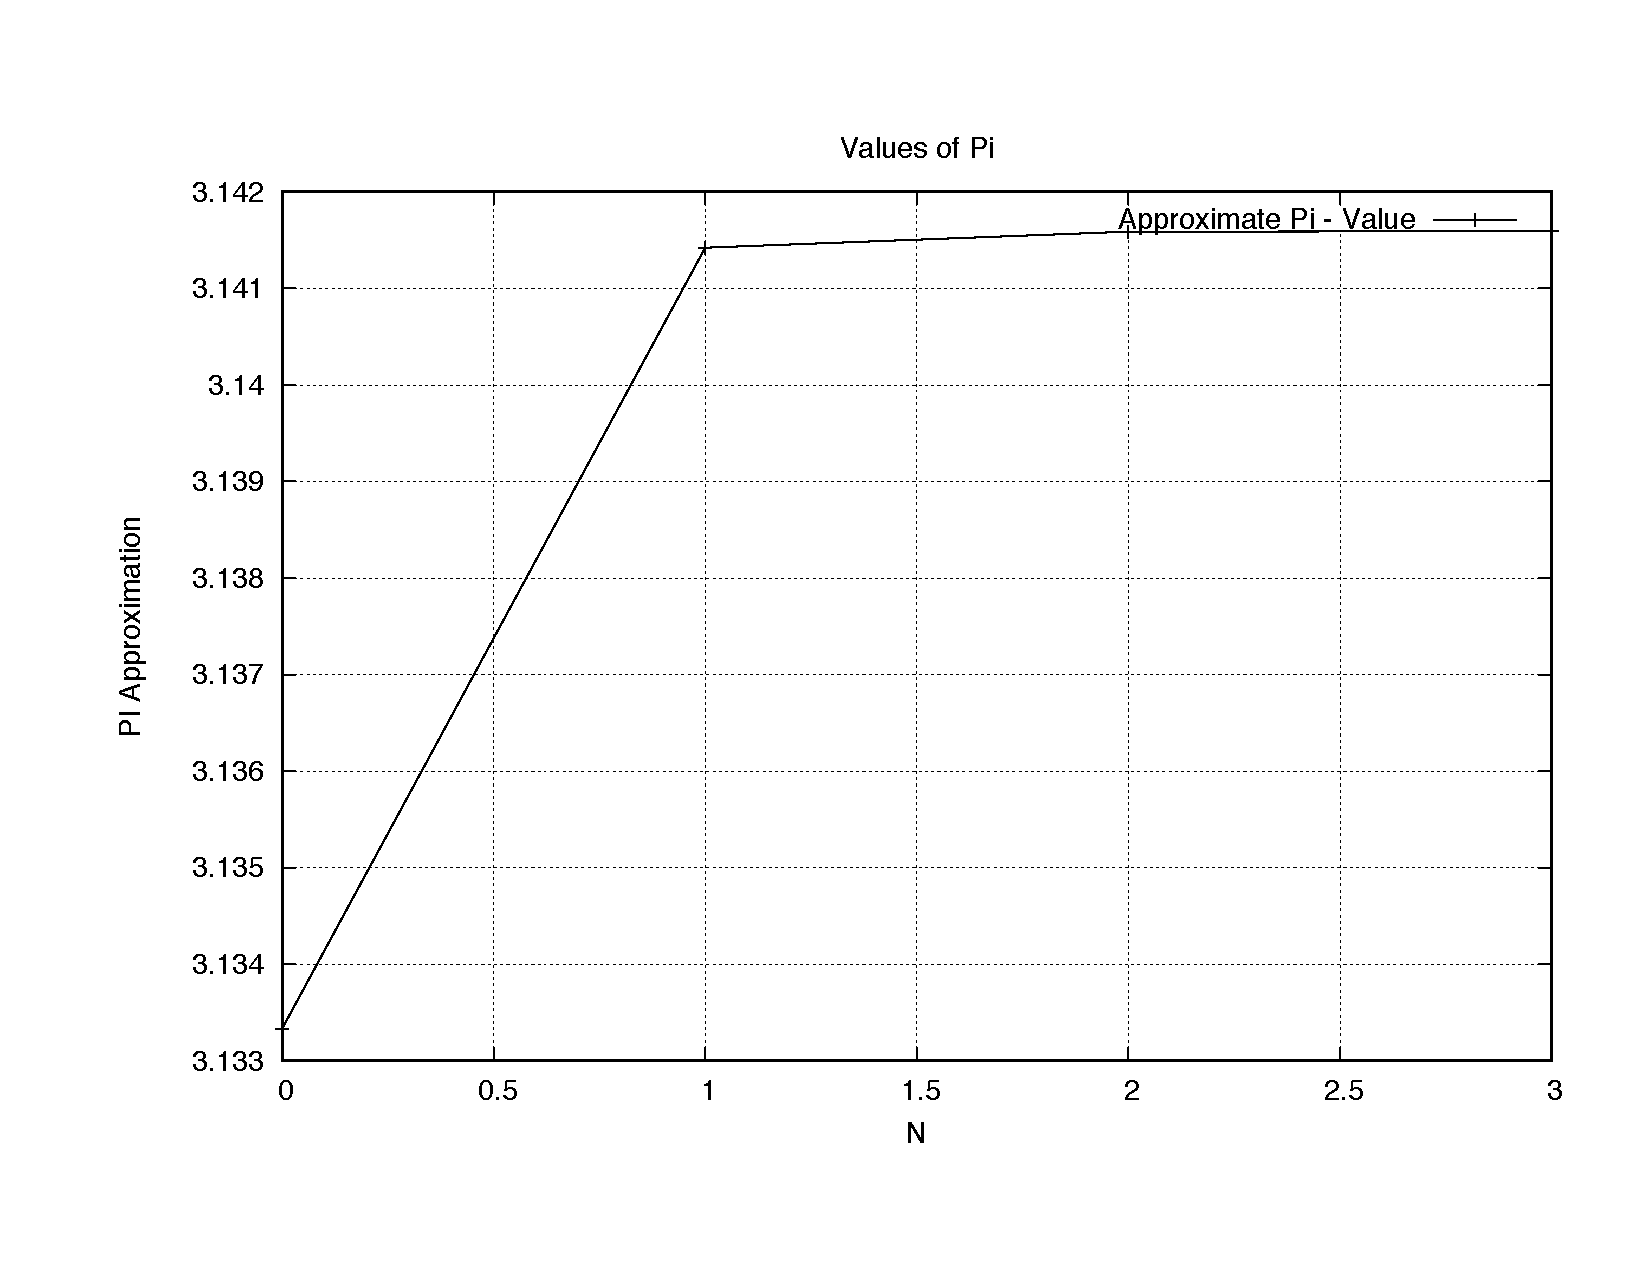
\includegraphics[width=0.85\textwidth]{./prob3/plots/pi_value.pdf}
				\label{fig:pi}
			\end{figure}












\end{document}